\chapter{Realizacja projektu}
%_______________________________________________________________________________________________________________
\section{Część sprzętowa}
\subsection{Przerzutka }
 Zasada działania serwomechanizmu kontrolującego pozycję wózka została przedstawina na rys. \ref{fig:przerzutkaSerwo}. Zmiana pozycji wału serwomechazmu implikuje zmianę pozycji wózka poprzez zastosowanie sztywnego połączenia przegłubowego.
 \begin{figure}[h]
    \centering
    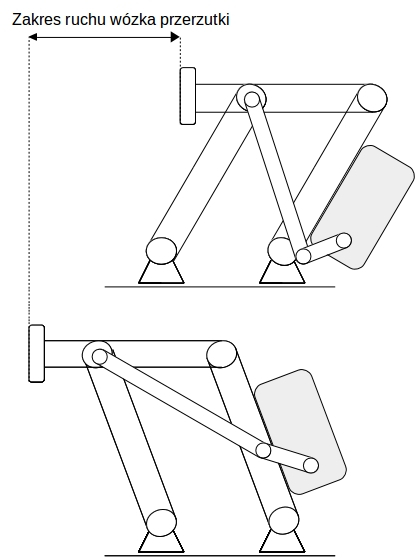
\includegraphics[scale=0.5]{przerzutkaSerwo.jpg}
    \caption{Zasada działania przerzutki rowerowej z wykorzystaniem serwomechanizmu}
    \label{fig:przerzutkaSerwo}
\end{figure}

Przymocowanie serwomechanizmu do przerzutki, zgodnie ze schematem przedstawionym na rys. \ref{fig:przerzutkaSerwo}  można podzielić na kilka etapów.
Pierwszy etap to usunięcie sprężyny, która występuje w konwencjonalnych przerzutkach tylnych. Wiąże się to ze zniszczeniem połączeń nitowych do których przymocowana jest sprężyna. Zniszczone połączenia nitowe zastąpione zostały przez połączenia śrubowe. Wykorzystane zostały śruby z gwintem metrycznym M4 o średnicy 4 mm.

Następny etap to wykonanie elementu mocującego serwomechanizm do przerzutki. Element został wykonany zgodnie z projektem przedstawionym na rysunku technicznym:.\textcolor{red}{@TODO rysunek}.

Wykonany element wraz z połączeniami śrubowymi umożliwa przymocowanie serwomechanizmu Hitec Hs-8335SH do przerzutki SRAM X5. Ostatni etap tej części projektu to wykonanie połączenia przegłubowego łączącego wał serwomechanizmu z jednym z członów ruchomych przerzutki. Autor zdecydwał się na zastosowanie modelarskiego drążka kierwoniczego o zmiennej długości oraz dedykowanego aluminowego orczyka serwomechanizmu. Takie rozwiązanie pozwala dokładnie dopasować długość  połączenia, bez konieczności projektowania oraz wykonania dodatkowych elementów.

W wyniku poywższych czynności powstała w pełni funkcjonalna przerzutka tylna sterowana przy użyciu serwomechanizmu. 

%_______________________________________________________________________________________________________________
\subsection{Integracja elementow elektronicznych}
Miktrokontroler, filtry RC, pakiet zasilający, regulator napięcia oraz jednostka pomiarowa IMU zamontowane zostały w hermetycznej puszcze elektrycznej, przymocowanej na stałe do dolnej rury przedniego trójkąta ramy rowerowej. Szczegłówy schemat połączeń znajduje się na rys. \textcolor{red}{SCHEMAT EAGLE}. Ze względu na rozwojowy charakter projektu oraz częste zmiany wprowadzane na etapie realizacji, autor pracy nie zdecydował się na wykonanie dedykowanego obwodu drukowanego.
%_______________________________________________________________________________________________________________

\section{Część programowa}
\subsection{Struktura programu}
Zasada działania programu przedstawiona zotała na rys. \ref{fig:schematAlgorytmu} i może zotać porównana do skończonej maszyny stanów. Autor rozważał wykorzystanie systemu czasu rzeczywistego \textit{freeRTOS}, w którym poszczególne stany będą odpowiadały nowym zadaniom, odpalanym sekwencyjnie. Jednak właśnie ze względu na sekwencyjne wykonywanie głównych zadań oraz brak ostrych wymagań czasowych, pomysł ten został odrzucony. Dlatego porównanie zasady działanai programu do skończonej maszyny stanów ma na celu jedynie zilustrowanie zasady jego działania.

Cel pracy to wykonanie układu zmiany przełożeń, który oferuje dwa tryby pracy - tryb ręczny oraz automatyczny. Autor zdecydował, że w ramach trybu automatycznego wykonany zostanie podział na tryb comfort, active i sport. Inspiracją  takiego rozwiązania jest branża motoryzacyjna, w której coraz częściej można spotkać układy automatycznej zmiany przełożeń, oferujące możliwość profilowania charakterystyki działania zmiany biegów, poprzez wybór jednego z trybów jazdy.
\begin{figure}[h]
    \centering
    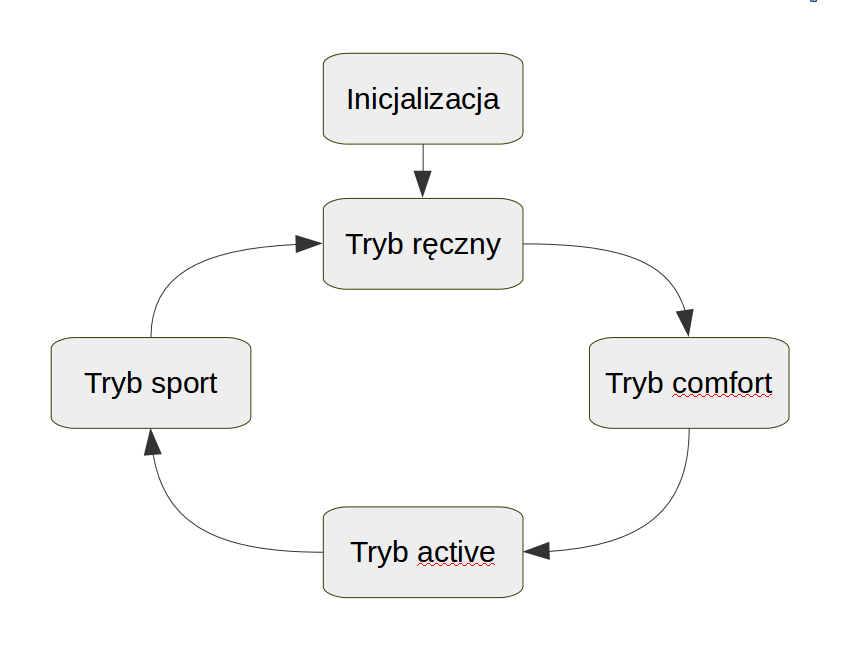
\includegraphics[scale=0.3]{schematAlgorytmu.png}
    \caption{Schemat ilustrujący zasadę działania programu kontrolera}
    \label{fig:schematAlgorytmu}
\end{figure}
\subsubsection{Inicjalizacja peryferiów}
Stan inicjalizacji jest stanem początkowym programu, osiąganym jednokrotnie po włączeniu zasilania. W tym stanie następuje inicjalizacja wszystkich układów peryferyjnych. 

Inicjalizowane są:
\begin{itemize}
\item
Porty wejściowe odpowiedzialne za obsługę przycisków do zmiany przełożeń oraz czujników magnetycznych.
\item
Porty wyjściowe odpowiedzialne za generowanie sygnału sterującego serwomechanizmem oraz sterowanie wstaźnikiem RGB aktualnego stanu programu. 
\item
Inercyjna jednostka pomiarowa
\item
Układy czasowo licznikowe, które inicjują zadania okresowe oraz wykorzystywane są do pomiaru prędkości obrotowej i kadencji
\end{itemize}

W przypadku, gdy inicjalizacja wszystkich układów przebiegnie bez błędów, następuje przejście do nastepnego stanu - tryb ręczny.
\subsubsection{Tryb ręczny}
Tryb ręczny jest pierwszym stanem, w którym użytkownik może korzystać z funkcjonalności układu zmiany przełożeń. Zasada działania odpowiada w pełni mechanicznemu układowi. W tym trybie obsługiwane są jedynie przyciski do zmiany przełożeń. Oprogramowanie umożliwia jednokrotną zmianę przełożenia, aktywowaną poprzez naciśnięcie odpowiedniego przycisku. Dodatkowo zaimplementowana została ciągła zmiana przełożeń, która uruchamiana jest poprzez naciśnięcie i przytrzymanie odpowiedniego przycisku. Przełożenia zmieniane są co 1 sekundę, więc użytkownik ma odpowiedniu dużo czasu do zatrzymania zmiany na odpowiednim przełożeniu.

Naciśnięcie przycisku zmiany trybu pracy układu powoduje przejście do kolejnego stanu - trybu comfort.

\subsubsection{Tryb comfort}
Stan comfort jest pierwszym z zaimplementowanych trybów automatycznej zmiany przełożeń. Ten tryb jest przeznaczony do spokojnego przemieszczania się na rowerze po płaskim terenie. Jest to najprostszy z trybów automatycznych, który nie powinien angażować użytkownika do podejmowania żadnych decyzji. Możliwość zmiany ręcznej jest wyłączona. Mierzona jest jedynie chwilowa wartość kadencji. Płaski charakter trasy sprawia, że cykliczne zadanie, w trakcie którego dobierane jest przełożenie, zależne od wartości kadencji, uruchamiane jest z niską częstotliwością. Zakres kadencji jest stały dla każdego przełożenia i dobrany w taki sposób, aby umożliwić spokojną i komfortową jazdę na rowerze.  

\subsubsection{Tryb active}
\subsubsection{Tryb sport}  
 


\subsubsection{Tryb manualny}
%_______________________________________________________________________________________________________________

\subsection{Szczegóły implementacji}


%_______________________________________________________________________________________________________________
\subsubsection{Kontrola serwomechanizmu}
%_______________________________________________________________________________________________________________
\subsubsection{Obsługa przycisków}
%_______________________________________________________________________________________________________________
\subsubsection{Kontrola zbliżeniowych czujników magnetycznych}
%_______________________________________________________________________________________________________________
\subsubsection{Obsługa Pololu AltIMU10}
%_______________________________________________________________________________________________________________




